\begin{figure}[!ht]
    \centering
    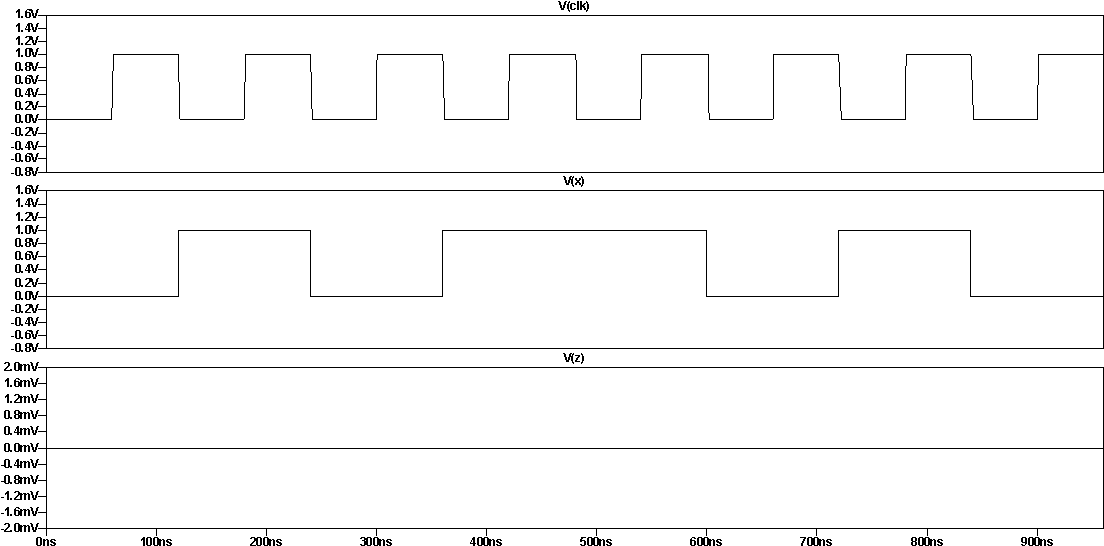
\includegraphics[width=0.9\textwidth]{inc/Q/Q11/Q11.pdf}
    \caption{LTspice Simulation Traces V(CLK), V(X) and V(Z) for Q11}\label{fig:Q11}
\end{figure}\FloatBarrier 

    Figure~\ref{fig:Q11} shows the output V(Z) as a flat line indicating the circuit is not operating correctly due to being clocked too fast.

    V(X) clocked on the falling edge of V(CLK) and V(Z) is clocked on the rising edge of V(CLK). This means any change in V(X) only has half a clock cycle to propagate to the the input of $D_{a}$. $t_{JHBCD} = 71ns$ which is more than half of the clock cycle (60ns) when $ t_{CLK} = 120ns $. This means the circuit is not operating correctly due to being clocked too fast.